\documentclass[a4paper, 12pt]{article}
\usepackage[utf8]{inputenc}
\usepackage[american]{babel}
\usepackage[margin=1in]{geometry}
\usepackage{mathtools}
\usepackage{fancyhdr}
\usepackage{tikz}
\usepackage{enumitem}
\usetikzlibrary{shapes, calc}
\setlength{\headheight}{15.2pt}
\pagestyle{fancy}
\lhead[]{Joseph Petitti}
\rhead[]{Homework 3}
\chead[]{Database Systems II}

\begin{document}

\section*{Problem 1}

\noindent After inserting 20:

\begin{center}
	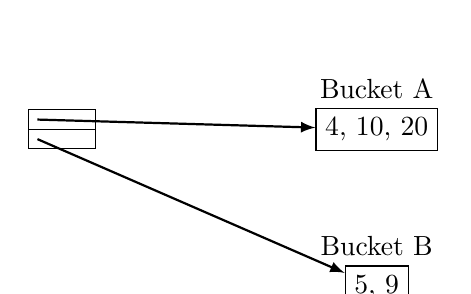
\begin{tikzpicture}
		\tikzstyle{bucket}=[rectangle, draw]
		\tikzstyle{left}=[rectangle, rectangle split, rectangle split parts=2]
		\tikzstyle{every node}=[bucket]

		\node[left] (root) {
			\nodepart{one} \hphantom{asdf}
			\nodepart{two} \hphantom{asdf}
		};

		\node[bucket, label={Bucket A}, right of=root, xshift=3cm] (bucketA) {
			4, 10, 20
		};

		\node[bucket, label={Bucket B}, below of=bucketA, yshift=-1cm] (bucketB) {
			5, 9
		};

		\draw[->, thick, >=latex] (root.one) -- (bucketA);
		\draw[->, thick, >=latex] (root.two) -- (bucketB);

	\end{tikzpicture}
\end{center}

\noindent After inserting 33:

\begin{center}
	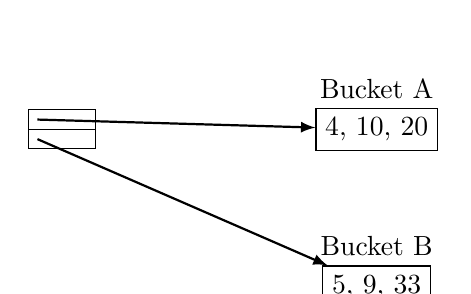
\begin{tikzpicture}
		\tikzstyle{bucket}=[rectangle, draw]
		\tikzstyle{left}=[rectangle, rectangle split, rectangle split parts=2]
		\tikzstyle{every node}=[bucket]

		\node[left] (root) {
			\nodepart{one} \hphantom{asdf}
			\nodepart{two} \hphantom{asdf}
		};

		\node[bucket, label={Bucket A}, right of=root, xshift=3cm] (bucketA) {
			4, 10, 20
		};

		\node[bucket, label={Bucket B}, below of=bucketA, yshift=-1cm] (bucketB) {
			5, 9, 33
		};

		\draw[->, thick, >=latex] (root.one) -- (bucketA);
		\draw[->, thick, >=latex] (root.two) -- (bucketB);

	\end{tikzpicture}
\end{center}

\noindent After inserting 13:

\begin{center}
	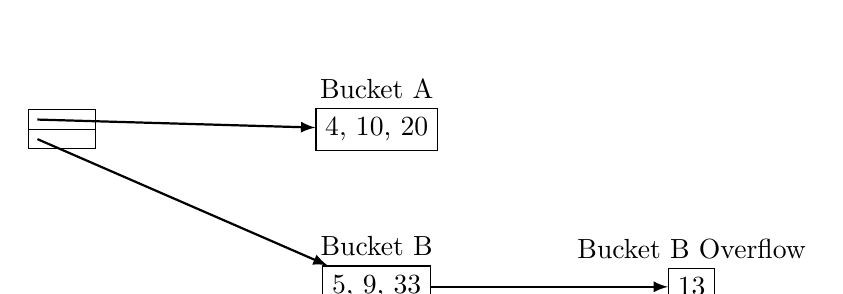
\begin{tikzpicture}
		\tikzstyle{bucket}=[rectangle, draw]
		\tikzstyle{left}=[rectangle, rectangle split, rectangle split parts=2]
		\tikzstyle{every node}=[bucket]

		\node[left] (root) {
			\nodepart{one} \hphantom{asdf}
			\nodepart{two} \hphantom{asdf}
		};

		\node[bucket, label={Bucket A}, right of=root, xshift=3cm] (bucketA) {
			4, 10, 20
		};

		\node[bucket, label={Bucket B}, below of=bucketA, yshift=-1cm] (bucketB) {
			5, 9, 33
		};

		\node[bucket, label={Bucket B Overflow}, right of=bucketB, xshift=3cm]
		(bucketBOverflow) {
			13
		};

		\draw[->, thick, >=latex] (root.one) -- (bucketA);
		\draw[->, thick, >=latex] (root.two) -- (bucketB);
		\draw[->, thick, >=latex] (bucketB) -- (bucketBOverflow);

	\end{tikzpicture}
\end{center}

\noindent After inserting 14:

\begin{center}
	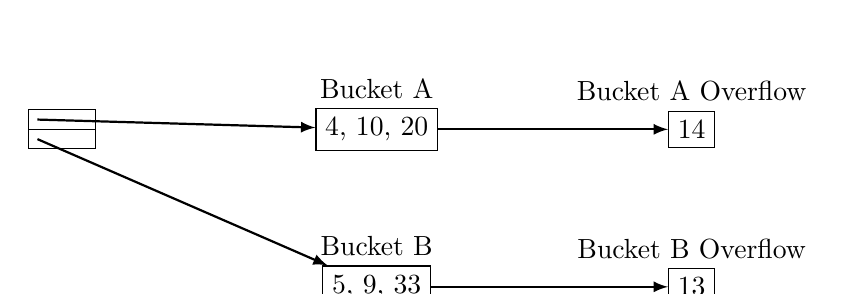
\begin{tikzpicture}
		\tikzstyle{bucket}=[rectangle, draw]
		\tikzstyle{left}=[rectangle, rectangle split, rectangle split parts=2]
		\tikzstyle{every node}=[bucket]

		\node[left] (root) {
			\nodepart{one} \hphantom{asdf}
			\nodepart{two} \hphantom{asdf}
		};

		\node[bucket, label={Bucket A}, right of=root, xshift=3cm] (bucketA) {
			4, 10, 20
		};

		\node[bucket, label={Bucket B}, below of=bucketA, yshift=-1cm] (bucketB) {
			5, 9, 33
		};

		\node[bucket, label={Bucket A Overflow}, right of=bucketA, xshift=3cm]
		(bucketAOverflow) {
			14
		};

		\node[bucket, label={Bucket B Overflow}, right of=bucketB, xshift=3cm]
		(bucketBOverflow) {
			13
		};

		\draw[->, thick, >=latex] (root.one) -- (bucketA);
		\draw[->, thick, >=latex] (root.two) -- (bucketB);
		\draw[->, thick, >=latex] (bucketB) -- (bucketBOverflow);
		\draw[->, thick, >=latex] (bucketA) -- (bucketAOverflow);

	\end{tikzpicture}
\end{center}

\section*{Problem 2}

\subsection*{1}

\begin{enumerate}[label=(\alph*)]
	\item Non-blocking, because it can output tuples as it processes inputs, and
		just won't output them again if it has encountered the same tuple
		before.
	\item Non-blocking. If column X is sorted, once it finds a different value
		of X it can output all tuples of the previous value because they make up
		an entire group.
	\item Blocking, because it needs to find all elements in a specific group
		before it can start outputing them.
	\item Blocking, because it needs to process all tuples in R before it can
		output the sorted list of tuples.
	\item Non-blocking. Since the leaves of the B-tree are already sorted it can
		just output them in order as it reads them in.
	\item Blocking, because it must first sort R and S, and then merge join
		them.
	\item Non-blocking, it can output the resulting tuples as it reads in the
		input.
\end{enumerate}

\subsection*{2}

\begin{enumerate}[label=(\alph*)]
	\item Can be done in one pass assuming the distinct tuples of R fit in 199
		buffers.
	\item Can be done in one pass as long as the biggest group can fit in 199
		buffers.
	\item Can be done in one pass as long as R can fit in 199 buffers.
	\item Cannot be done in one pass. A two-pass external sort reads M blocks at
		a time, sorts them, and writes them to the disk as the first run, then
		merges the runs to produce a sorted output. The I/O cost will be $ 2
		\times B(R) $ for the first pass and $ B(R) $ for the second pass, for a
		total of $ 3 B(R) = 3 \times 1000 = 3000 $ I/Os.
	\item Can be done in one pass, with 70 I/Os to read the index, plus 2000
		I/Os to read and write the sorted relation R, for a total of 2070 I/Os.
	\item Cannot be done in one pass. Phase one can sort R and S, while phase
		two merges and joins the sorted relations R and S. The I/O cost is $ 2
		\times B(R) + 2 \times B(S) $ for phase one sorting, plus $ B(R) + B(S)
		$ for the merge and join phase two, for a total cost of $ 3 ( B(R) +
		B(S)) = 3 ( 1000 + 150 ) = 3450 $ I/Os.
	\item Can be done in one pass because S can fit in 199 buffers.
\end{enumerate}

\section*{Problem 3}

\begin{enumerate}
	\item $ Q = T(R1) / V(R1_a) = 400 / 50 = 8 $
	\item $ Q = \left ( \frac{T(R1)}{V(R1_a)} \right ) \times 41 = 328 $
	\item $ Q = 328 \times (1 / 50) = 7 $
	\item $ Q = T(R1) \times T(R2) \div \text{max}(V(R1_b), V(R2_b)) = 400
		\times 500 \div \text{max}(50, 40) = 4000 $
	\item $ Q = 4000 \times T(R3) \div \text{max}(V(R2_c), V(R3_c)) = 4000
		\times 1000 \div 100 = 40000 $
	\item $ Q = ( 328 \bowtie R2 ) \bowtie R3 = ( 328 \times 500 \div 50 )
		\bowtie R3 = 3280 \bowtie R3 = 3280 \times 1000 \div 100 = 32800 $
\end{enumerate}

\section*{Problem 4}

\begin{enumerate}
	\item
		\begin{enumerate}[label=\alph*.]
			\item R2, because it's smaller
			\item $ B(R2) + \frac{B(R2)}{M - 1} \times B(R1) = 200 +
				\frac{200}{51} \times 1000 = 4122 $ IOs
			\item $ B(R1) + \frac{B(R1)}{M - 1} \times B(R2) = 1000 +
				\frac{1000}{51} \times 200 = 4922 $ IOs
		\end{enumerate}

	\item
		\begin{enumerate}[label=\alph*.]
			\item $ 3 (B(R1) + B(R2)) = 3 (1000 + 200) = 3600 $
			\item $ B(R1) + B(R2) \leq M^2 $

				$ 1000 + 200 \leq M^2 $

				$ M >= 34 $

				Minimum number of buffers necessary is 34	
		\end{enumerate}

	\item
		\begin{enumerate}[label=\alph*.]
			\item $ 3 (B(R1) + B(R2)) = 3 (1000 + 200) = 3600 $
			\item $ B(R2) \leq M^2 $

				$ 200 \leq M^2 $

				$ M >= 14 $

				Minimum number of buffers is 14
		\end{enumerate}

	\item
		\begin{enumerate}[label=\alph*.]
			\item Assuming R2 is clusteded, R1.a index is in memory, and the
				index is clustered.

				$ B(R2) + T(R2) \times (B(R1) / V(R1,a)) = 200 + 2000 \times (
				1000 / 500 ) = 4200 $
		\end{enumerate}
\end{enumerate}

\end{document}
